\documentclass[pdftex,12pt,a4paper]{article}

\usepackage{graphicx}  
\usepackage[margin=2.5cm]{geometry}
\usepackage{breakcites}
\usepackage{indentfirst}
\usepackage{pgfgantt}
\usepackage{pdflscape}
\usepackage{float}
\usepackage{epsfig}
\usepackage{epstopdf}
\usepackage[cmex10]{amsmath}
\usepackage{stfloats}
\usepackage{multirow}

\renewcommand{\refname}{REFERENCES}
\linespread{1.3}

\usepackage{mathtools}
%\newcommand{\HRule}{\rule{\linewidth}{0.5mm}}
\thispagestyle{empty}
\begin{document}
\begin{titlepage}
\begin{center}
\textbf{}\\
\textbf{\Large{ISTANBUL TECHNICAL UNIVERSITY}}\\
\vspace{0.5cm}
\textbf{\Large{COMPUTER ENGINEERING DEPARTMENT}}\\
\vspace{2cm}
\textbf{\Large{BLG 242E\\ DIGITAL CIRCUITS LABORATORY\\ EXPERIMENT REPORT}}\\
\vspace{2.8cm}
\begin{table}[ht]
\centering
\Large{
\begin{tabular}{lcl}
\textbf{EXPERIMENT NO}  & : & 1 \\
\textbf{EXPERIMENT DATE}  & : & 14.02.2020 \\
\textbf{LAB SESSION}  & : & FRIDAY - 08.30 \\
\textbf{GROUP NO}  & : & G14 \\
\end{tabular}}
\end{table}
\vspace{1cm}
\textbf{\Large{GROUP MEMBERS:}}\\
\begin{table}[ht]
\centering
\Large{
\begin{tabular}{rcl}
150180082  & : & TEVFIK \& OZGU \\
150170017  & : & CEYHUN \& UGUR \\
150190739  & : & YASIN ABDULKADIR \& YOKUS \\
\end{tabular}}
\end{table}
\vspace{2.8cm}
\textbf{\Large{SPRING 2020}}

\end{center}

\end{titlepage}


\thispagestyle{empty}
\addtocontents{toc}{\contentsline {section}{\numberline {}FRONT COVER}{}}
\addtocontents{toc}{\contentsline {section}{\numberline {}CONTENTS}{}}
\setcounter{tocdepth}{4}
\tableofcontents
\clearpage

\setcounter{page}{1}

\section{INTRODUCTION [10 points]}

For this laboratory section, it is expected to make 5 experiments. So we used CADET, Voltmeter, the function generator, and the oscilloscope device. Since it is the first week, it was aimed to teach how to use these devices and it is expected from students to recognize some basic gate properties. 

\section{MATERIALS AND METHODS [40 points]}
In order to conduct Experiment – I, these tools are needed:

\begin{itemize}
    \item C.A.D.E.T (Complete Analogue Digital Electronic Trainer)
        \begin{figure}[ht]
    	\centering
    	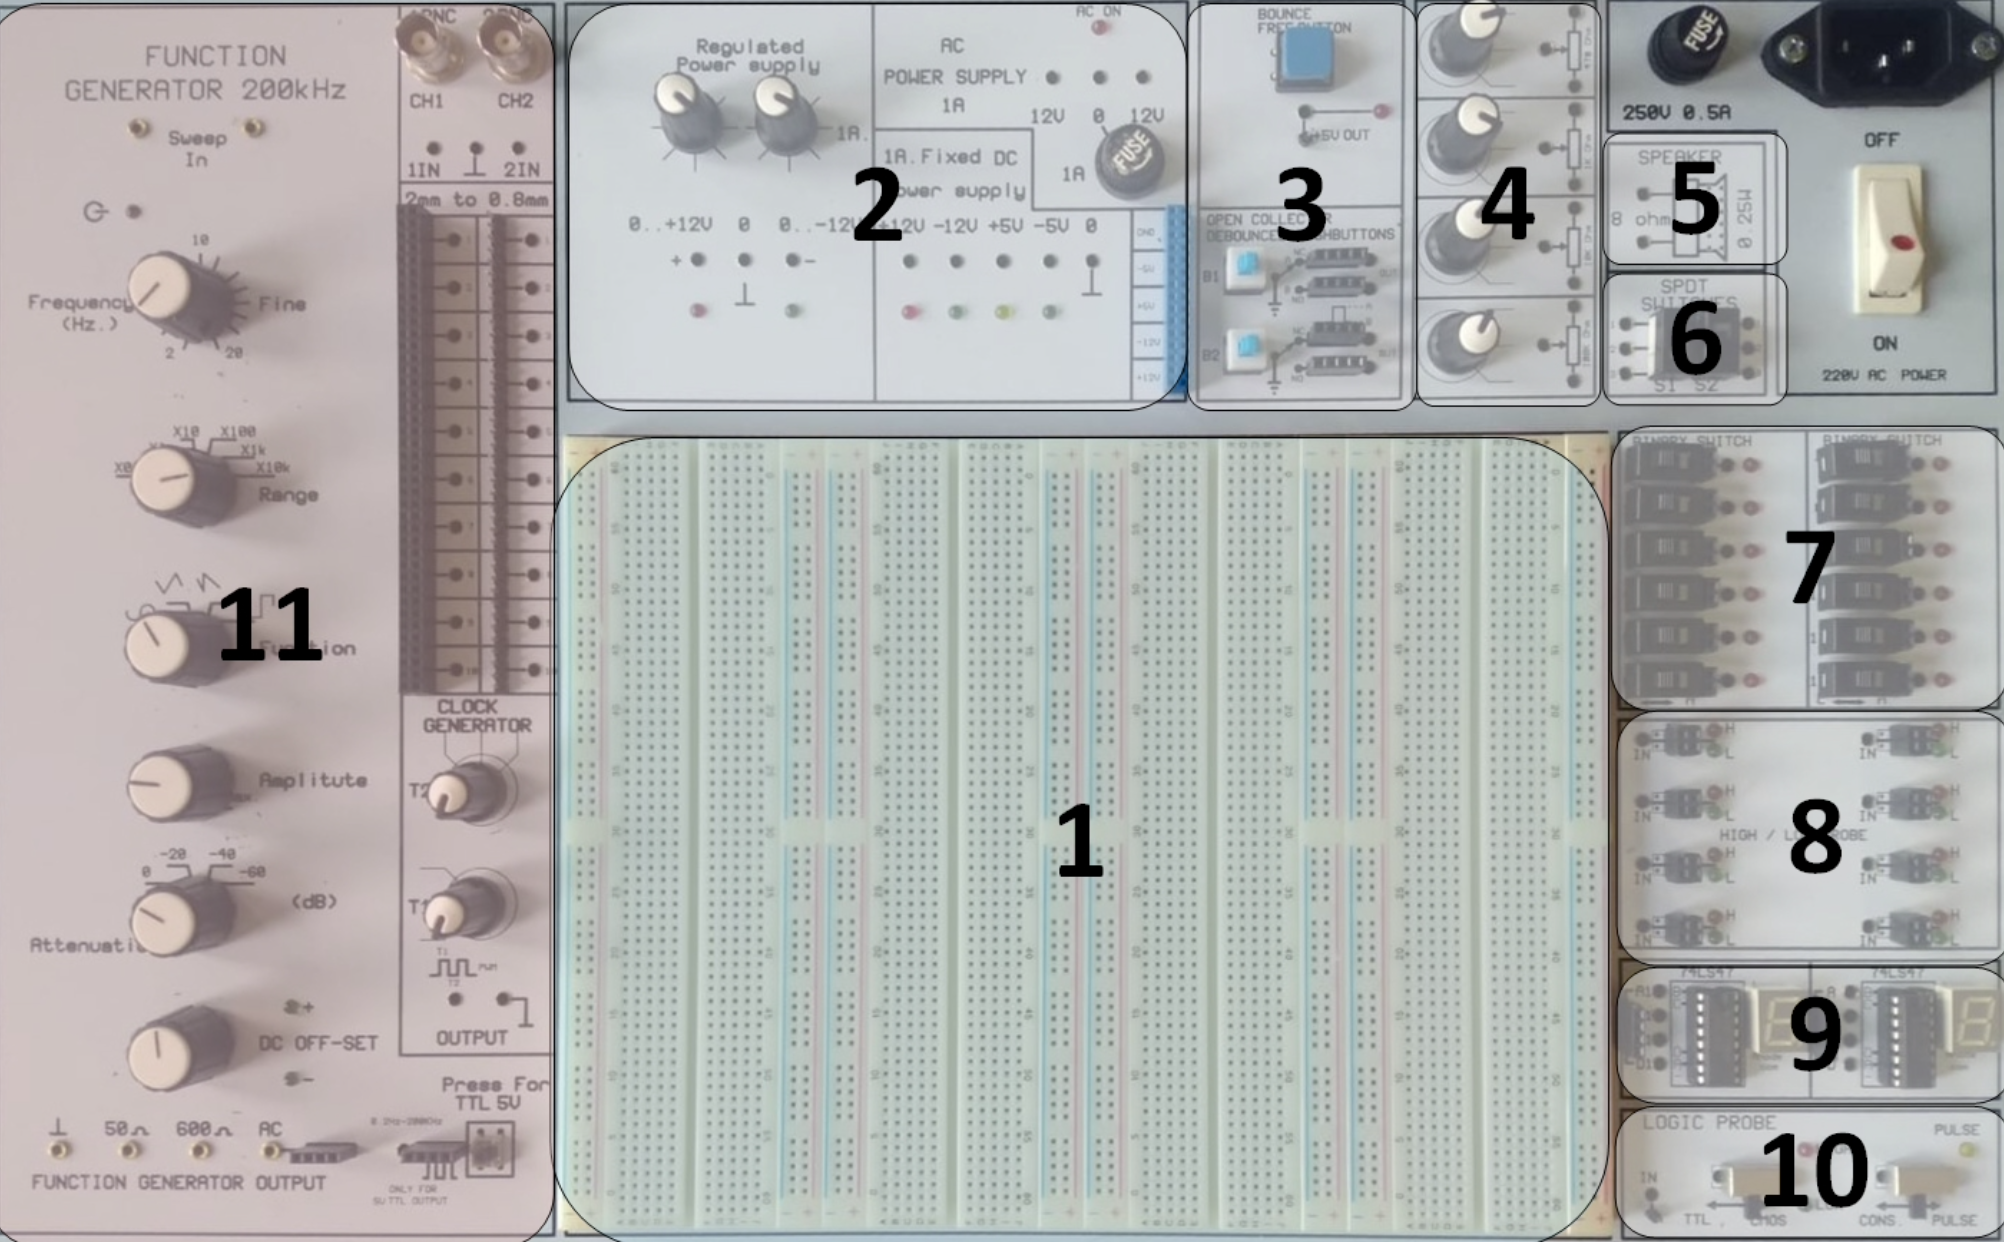
\includegraphics[width=1\textwidth]{CADET.png}	
    	\caption{C.A.D.E.T. Device\cite{ref1}}
    	\label{fig2}
        \end{figure}
    \newpage
    \item Function Generator
    \begin{figure}[ht]
    	\centering
    	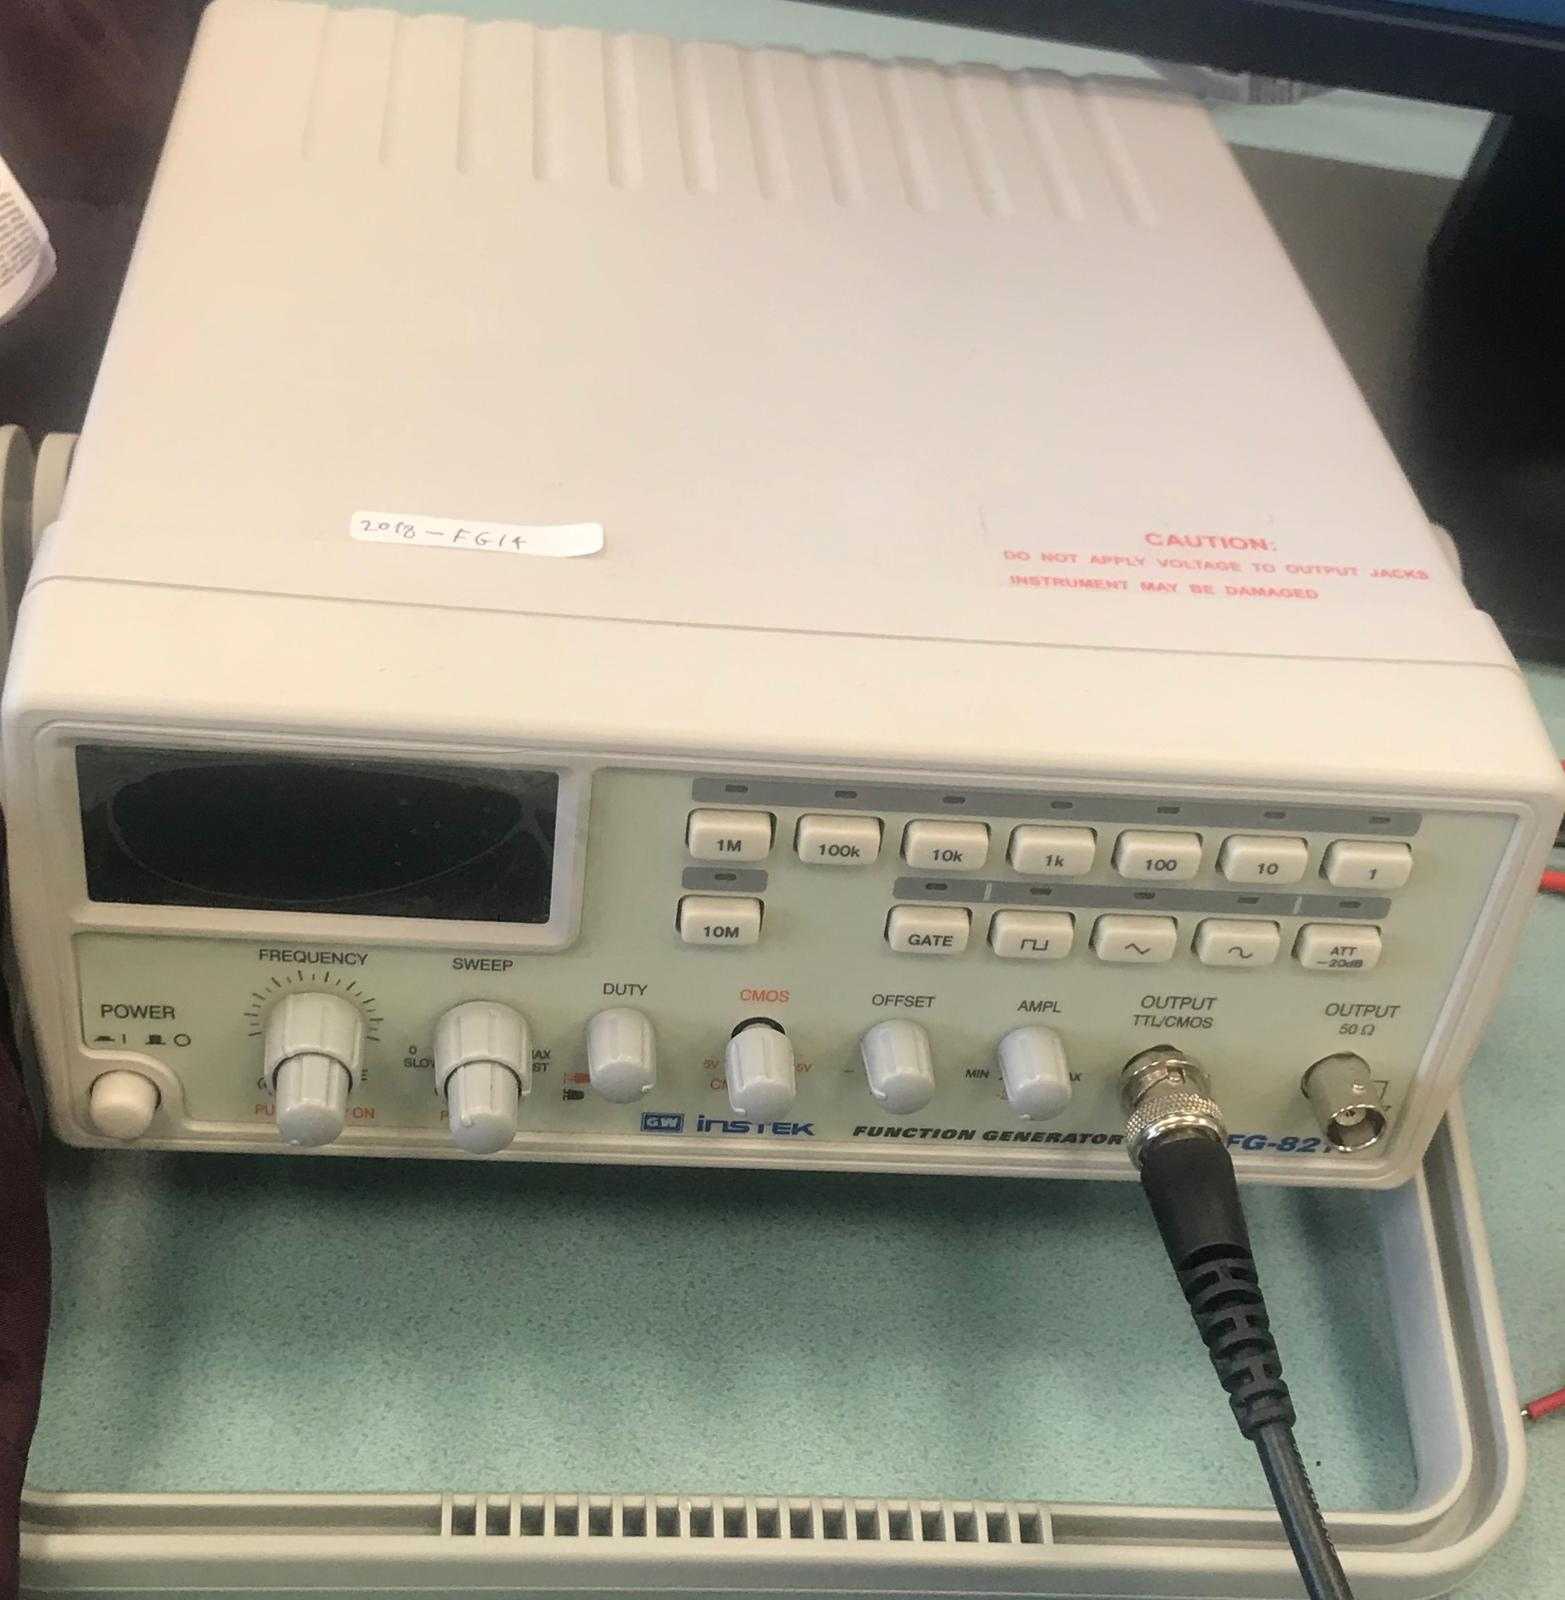
\includegraphics[width=0.8\textwidth]{funcGen.jpeg}	
    	\caption{Function Generator}
    	\label{fig6}
        \end{figure}
    \newpage
    \item Oscilloscope
        \begin{figure}[H]
        	\centering
        	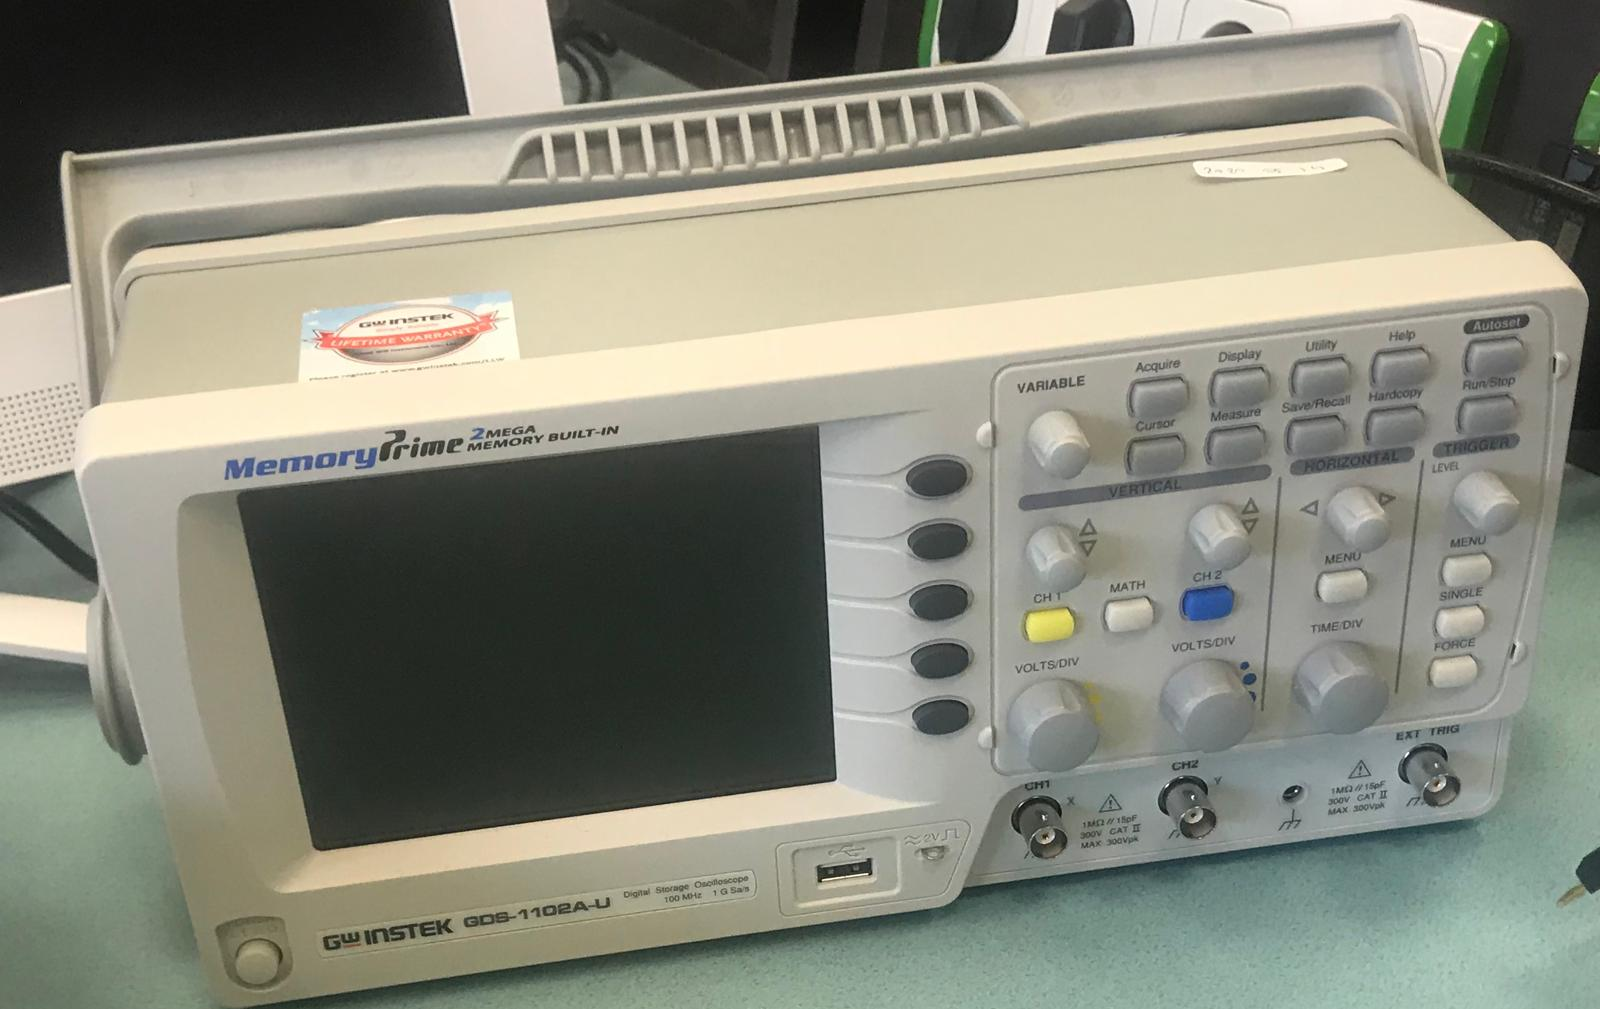
\includegraphics[width=0.8\textwidth]{osc.jpeg}	
        	\caption{Oscilloscope}
        	\label{fig7}
            \end{figure}
    \item 74000 series ICs
    \begin{itemize}
        \item 74x$x^{1}$04 - Hex Inverter
            \begin{figure}[ht]
        	\centering
        	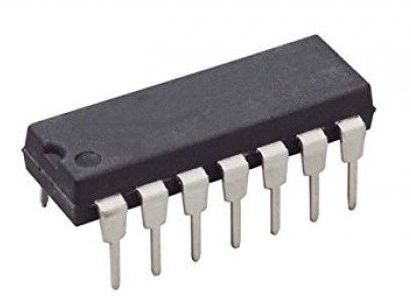
\includegraphics[width=0.2\textwidth]{7404.JPEG}
        	\caption{Inverter}
        	\label{fig8}
            \end{figure}
    \end{itemize}
    \item Connection cables
    \item Voltmeter
    
     \begin{figure}[ht]
        	\centering
        	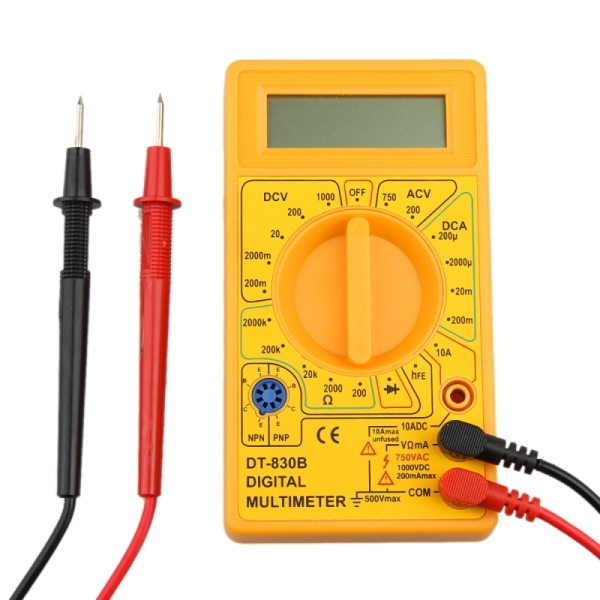
\includegraphics[width=0.2\textwidth]{voltmeter.jpg}
        	\caption{Voltmeter}
        	\label{fig9}
            \end{figure}
\end{itemize}

\newpage
\subsection{Experiment Part 1}
For this experiment, we used 4 wires. First wire is connected from the 2nd part of CADET’s ground also known as 0V to CADET’S power strip. But it is connected to - sign power strip. Other wire is connected form 5V to + power strip. Other wires is used for showing if it is High(5V) or Low(0V). First wire is connected from the used - power strip to one of the display in part 8 and other wire is connected from  the used + power strip to any other display of part 8. We saw that the light which was connected to - power strip is green namely Low(0) and other screen which is connected to + power strip is Red namely High(1).

\begin{figure}[ht]
	\centering
	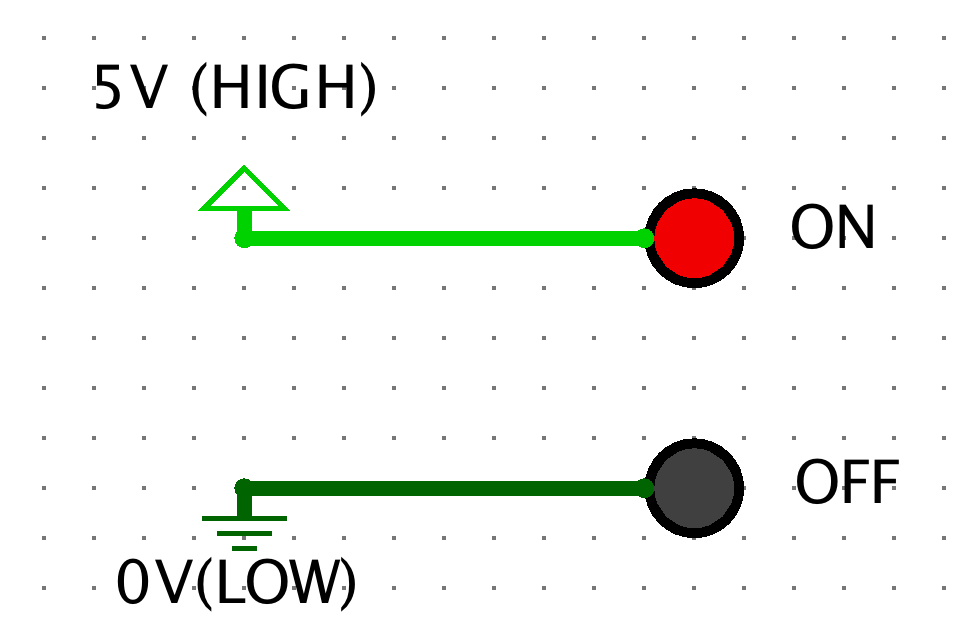
\includegraphics[width=0.5\textwidth]{part1.png}
	\caption{Power Display}
	\label{fig0}
	
\end{figure}

\subsection{Experiment Part 2}
In this part of the experiment we designed a circuit to implement a function which inverts the input using 7404 hex inverter. Firstly, we connected cables from power supply to power strips. Then we placed 7404 Hex Inverter to the breadboard. We connected cables from power strips to Vcc and ground which is shown on 7404 Hex Inverter Manual. We used 5V as Vcc and 0V as ground. Since horizontal holes are electrically same and named power strips, we placed another cable to one of horizontal input holes, then connected same cable to switch 1 of SPDT. Then we connected another cable to Inverted output and connected another end to switch 3 of SPDT. 

These two SPDT switches are intended for sending two alternative voltages to an output (i.e. switch 2). At last step we connected switch 2 (middle one) of SPDT to one of logic monitor LEDs which is receiving the voltage value of the different switches of SPDT through number 2 switch (i.e. output). Then we turned the SPDT switch up and down and we saw High and Low values at logic monitor LED, which indicate our input at one position and inverted input (i.e. output) at other position. Low at position 3 of SPDT (i.e. output) and High at position 1 of SPDT switch (i.e. input).
\begin{figure}[ht]
	\centering
	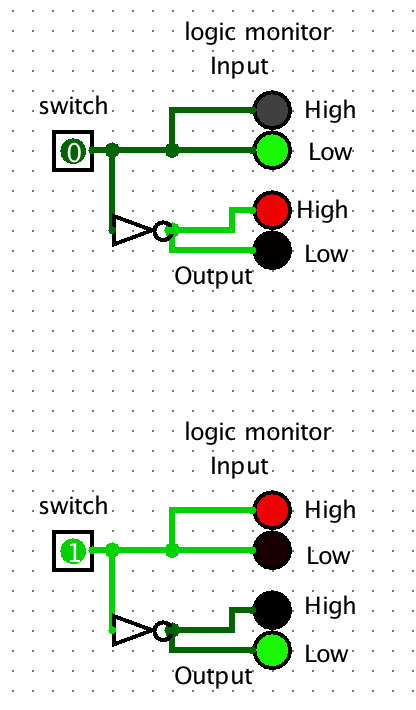
\includegraphics[width=0.5\textwidth]{switch.png}
	\caption{Representation Of Inverter by Switch}
	\label{fig1}
	
\end{figure}

\subsection{Experiment Part 3}
For this experiment, we used 4 wires. First wire is connected from the Power Supply of CADET’s ground also known as 0V to CADET’S power strip. But it is connected to - sign power strip. Other wire is connected form 5V to + power strip. Other wires is used for showing if it is High(5V) or Low(0V). First wire is connected from the used - power strip to one of the display in Logic Monitor and other wire is connected from  the used + power strip to any other display of Logic Monitor. We saw that the light which was connected to - power strip is green namely Low(0) and other screen which is connected to + power strip is Red namely High(1). 

\newpage
\subsection{Experiment Part 4}
To show 27 on the screen, we used binary to decimal converter. We connected 4 wires one by one from part 7 from CADET to displays. And we did it for second portion of this parts. So we handled 2 binary to decimal converter. First screen of decimal converter must show 2 and other screen must show 7. Decimal 2 is 0010 and decimal 7 is 0111. So in the first portion of part 7 we made R2 on and let others closed. So we showed 2 on the first screen of displays. In the other portion, we turned R1, R2 and R3 on than R4 is off. So we handled 7 on the second screen of displays. It has become 27.
\begin{figure}[ht]
	\centering
	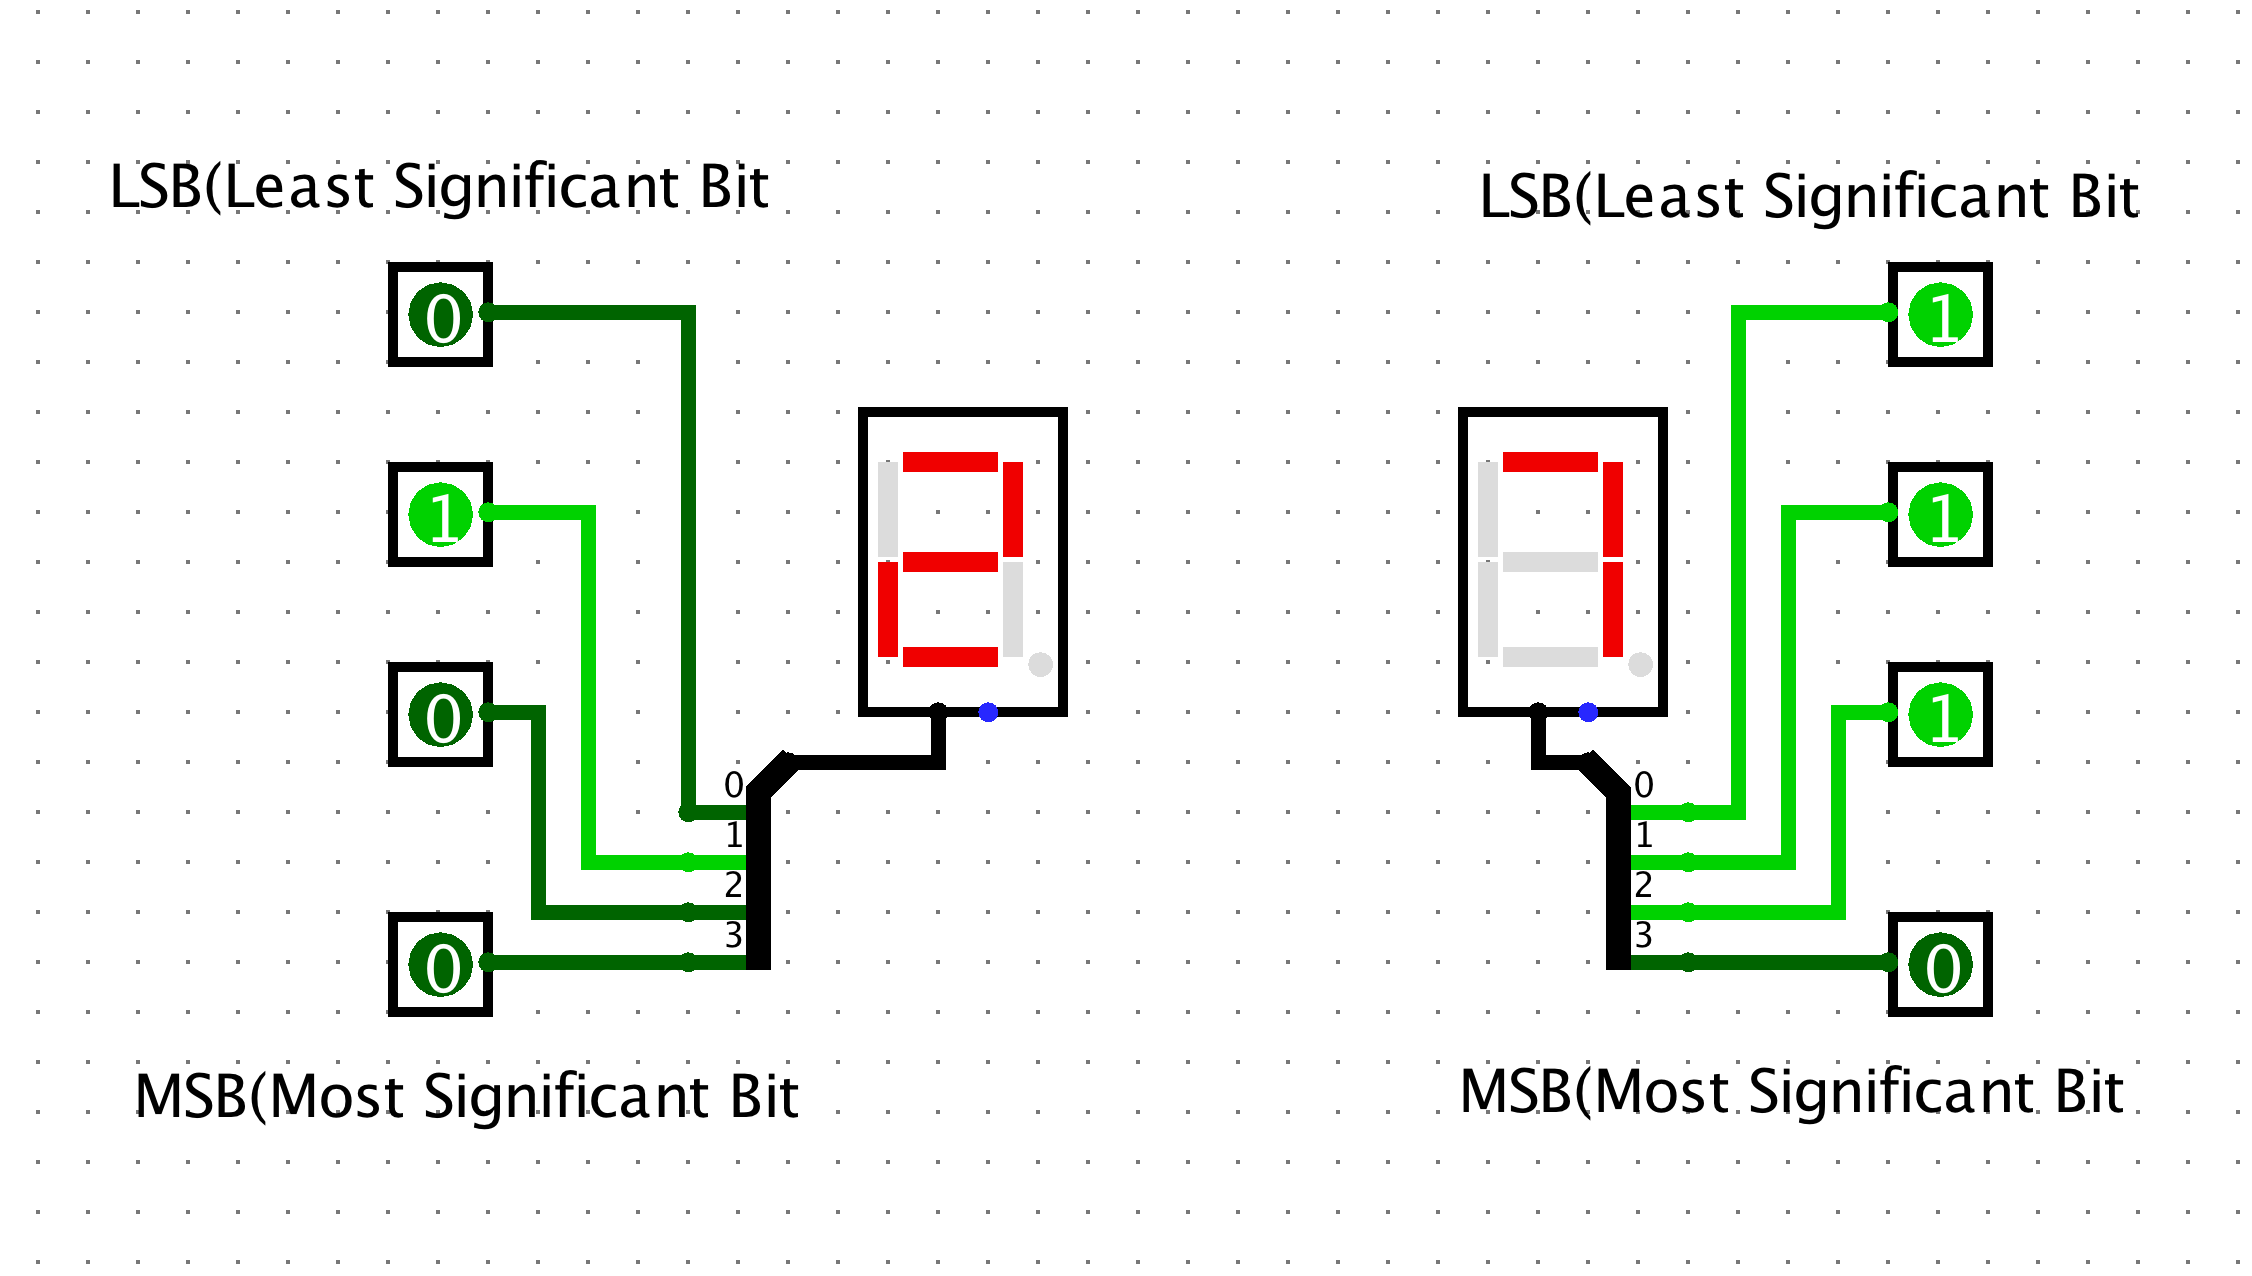
\includegraphics[width=0.6\textwidth]{27.png}
	\caption{Way to represent 27 with by coding}
	\label{fig3}
\end{figure}

\subsection{Experiment Part 5}

In the final part of the experiment, we produced some waves with different frequencies
and voltages using function generator then we observed these waves on oscilloscope.

\subsubsection{27 kHz TTL}

Firstly we set the range selector to 100k on the function generator. Then we adjusted frequency to 27 kHz with the frequency slider. We didn't touch anything for the voltage because TTL always produces 5V square wave as output.

\subsubsection{5 V (Vpp), 1992 Hz CMOS}

We set the range selector to 10k on the function generator. Then we adjusted the voltage to 5 V because CMOS doesn't like TTL about that. CMOS output can range between 0.6 V and 15 V. Finally, we observed 1992 Hz CMOS wave.

\subsubsection{1 V (Vmax), 500 Hz CMOS}

We set the range selector to 1k on the function generator. Then we adjusted the maximum voltage to 1 V. Finally, we observed 500 Hz CMOS wave.

\subsubsection{3.14 V (Vpp), 0.6 MHz triangular wave}

In this part of the experiment, firstly we used the other output on the function generator. Thus, we could choose the triangular wave type. Then we adjusted the voltage to 3.14 V and we observed 0.6 MHz triangular wave.
\subsubsection{1.2 V (Vmax), sine wave with 2.5 ms period}

In this part of the experiment we also used the other output on the function generator which we could select the triangular wave type in the previous part. But this time we chose the sine wave type then we found 400 Hz frequency from the formula (P = 1/F). Finally, because of the relationship between Vmax and Vpp, to find the 1.2 V Vmax we set the Vpp to 2.4 V.
\subsubsection{0.7 V (Vpp), 0.001 GHz square wave}

We set the range selector to 10M on the function generator. Then we adjusted the Vpp to 0.7 V. As a result, we didn't touch to the output channel and we chose the square wave type. Then we
observed the wave on the oscilloscope.

\subsubsection{1250 mV (Vpp), 45 Hz square wave}
Like other sections, we changed our voltage to 1250 mV and we observed 45 Hz square wave. These are all done by function generator and observations taken from oscilloscope.


\newpage
\section{RESULTS [15 points]}
For every part of the experiment we observed some results. In the first part of experiment we understood that 5V is interpreted as High or numerically 1 in logic circuits and 0V is interpreted as Low or numerically 0. It is the way to give inputs to digital circuits. In the second part of the experiment, we built inverter circuit with switch button. Switch button was acting like multiplexer and it provides us to show inverted output in the display which was turned on by switch. In the 3rd part of the experiment Voltmeter is used to calculate the Gcc voltage and Vcc voltage. There was no surprise since Vcc is calculated as 5V and Gcc voltage is calculated as 0V. And thanks to Voltmeter and the potentiometer, we handled 8 K ohm resistance. In the 4rd part, we used CADET device to print 27 on the screen. We connected our circuit and we made first screen inputs 0010 and the second screen inputs 0111. So we get 27 on the screen. In the last part, we used function generator and oscilloscope to get the desired frequencies or voltages. We observed results on the oscilloscope.

\section{DISCUSSION [25 points]}
After brief explanation of teaching assistans on how to use laboratory tools like CADET, Function Generator, Oscilloscope and ICs, we started to design experiments part by part. 
Since we also studied the part which explains every tool we will be using during this semester from the experiment booklet , we successfully implemented every part of this experiment. However, on part 2 we had a brief discussion between group members on how to show the input and output of this inverter circuit seamlessly. Then we realized main purpose of SPDT is sending two alternative signals or voltages to an output.

Also at last part of the experiment which is part 5, we learned some differences between TTL and CMOS. 
For instance, CMOS output can range between 0.6 V and 15 V but TTL output gives a 5 V square wave.
We tried to see some different wave forms depend on different frequencies in the function generator. Also we could
produce different wave forms like square wave form, triangular wave form or sine wave form. Finally we studied 
about oscilloscope and we tried to observe specific waves depend on frequencies, voltages and output types.(TTL or CMOS)
In some part of the experiment we used Vpp, some part of the experiment we used Vmax and we changed it using the oscilloscope.


\section{CONCLUSION [10 points]}
Firstly it is very interesting to test informations which we learned theoretically from previous courses. We learned how to use CADET, oscilloscope, function generator and voltmeter. Also we learned how to connect circuits to each other. 4 experiments of this section was completely went as we expected but also there were some difficulties because of CADET and voltmeter connection properties. It is very good to  see that informations that we learned was totally running. We learned how to connect some transistors to CADET and how to connect some inputs to gate and get outputs from same gate. But part 5 was the part that exhausted us. It is because of the usage of function generator and oscilloscope. We succeed but we tried a lot and we learned how to use them. With the function generator we could generate TTL and CMOS functions, with CMOS we can generate different waves and we can change CMOS output voltage from 0.6V to 15V but TTL generates only square type wave and output voltage is 5V These experiments was really helpful to understand the basic of these devices and it is very good to test some gates. 


\newpage
\addcontentsline{toc}{section}{\numberline {}REFERENCES}

\nocite{overleaf}

\bibliographystyle{unsrt}
\bibliography{reference}

\end{document}

